\documentclass[a4paper,11pt,openany]{article}
\usepackage[utf8]{inputenc}
\usepackage[czech]{babel}
\usepackage{geometry}
\usepackage{tikz,multirow,listingsutf8,multicol,amsmath,amsfonts}
\lstset{showstringspaces=false,stringstyle=\color{orange},basicstyle=\ttfamily\large,keywordstyle=\bfseries\color{blue!60!black}}
\geometry{left=20mm,right=20mm,top=20mm,bottom=20mm}
\parindent=0mm
\parskip=0mm
\usepackage{lipsum}
\newcommand{\quotefont}[2]{
	#1 [online]. [Citováno \today].\\
	Dostupné z:\\\small \ttfamily #2 \normalfont
}
\newcommand{\float}{\texttt{float}}

\begin{document}
\begin{center}
\pagenumbering{arabic}
{\huge \textbf{(a,b)-stromy}}\\\vspace{\baselineskip}Zápočtová práce z Programování I pro pokročilé\\
\vspace{10mm} {\large Jiří Škrobánek\footnote[1]{Matematicko-fyzikální fakulta Univerzity Karlovy, {\ttfamily jiri@skrobanek.cz}}}\\
\vspace{10mm}\today, Ostrava
\end{center}
	
\section*{Abstract}
	
This documentation describes the entire functionality of (a,b)-trees implementation in Python 3 by Jiří Škrobánek. Aside from listing all methods, principles of (a,b)-trees are explained and complexity of used algorithms is analysed.
	
\tableofcontents
	
\section{Definice}
(a.b)-strom je strom. Musí platit $(a,b) \in \mathbb{N}^2, 2 \leq a, 2a - 1 \leq b $. (a,b)-strom je buďto prázdný, nebo mají všechny vnitřní vrcholy nejméně $a$ synů a nejvýše $b$ synů. Výjimkou je kořen, jenž musí mít mezi 2 a $b$ syny. Všechny listy leží v jedné hladiny. Vnějším vrcholům jsou přiřazeny unikátní klíče (prvky lineárně uspořádané množiny). Vnitřním vrcholům je přiřazen maximální klíč z jeho synů. Ve vnitřním vrcholu jsou uloženy klíče synů ve vzestupném pořadí. Pro každý podstrom platí, že mimo podstrom neexistují vnější vrcholy, které mají nižší klíč než maximální klíč v podstromu a zároveň vyšší klíč než minimální v~podstromu.
	
V tomto stromě se dá vyhledat vnější vrchol dle klíče v logaritmickém čase vzhledem k počtu vnějších vrcholů. Přidávání a odebírání listů rovněž funguje v logaritmickém čase.
	
Speciálním případem (a,b)-stromů $2a-1=b$ jsou B-stromy, mimo jiné oblíbený 2-3-strom.
	
\section{Metody}
Knihovna obsahuje třídy \texttt{InternalNode} a \texttt{ExternalNode} pro vnitřní a vnější vrcholy a třídu \texttt{ABTree}, která má metody popsané níže.
	
Počet vnějších vrcholů ve stromě značíme $E$.
	
\begin{lstlisting}[language=python,frame=none]
__init__(a: int,b: int)
\end{lstlisting}
Vytvoří (a,b)-strom pro konkrétní hodnoty $a,b$.
	
Výjimky: \texttt{ValueError}: Neplatná volba parametrů.
	
Složitost: $\mathcal{O}(1)$
\begin{lstlisting}[language=python,frame=none]
insert(self, key: int, value=None)
\end{lstlisting}
Vloží do stromu uspořádanou dvojici (key, value). Value může být libovolného typu nebo \texttt{None}.
	
Výjimky: \texttt{ValueError}: Strom již klíč obsahuje.
	
Složitost: $\Theta(\log(E))$
	
\begin{lstlisting}[language=python,frame=none]
delete(self, key: int)
\end{lstlisting}
Vymaže ze stromu vnější vrchol s klíčem \texttt{key}.
	
Výjimky: \texttt{ValueError}: Strom klíč neobsahuje.

Složitost: $\Theta(\log(E))$

\begin{lstlisting}[language=python,frame=none]
contains(self, key: int)
\end{lstlisting}
	
Vrací: \texttt{bool} Zda strom obsahuje daný klíč.

Složitost: $\Theta(\log(E))$
	
\begin{lstlisting}[language=python,frame=none]
find(self, key: int)
\end{lstlisting}
	
Vrací: Hodnotu ve vnějším vrcholu s daným klíčem.
	
Výjimky: \texttt{ValueError}: Strom klíč neobsahuje.
	
Složitost: $\Theta(\log(E))$
	
\begin{lstlisting}[language=python,frame=none]
item_count(self)
\end{lstlisting}
	
Vrací: \texttt{int} Počet vnějších vrcholů ve stromě.
	
Složitost: $\mathcal{O}(1)$
	
\begin{lstlisting}[language=python,frame=none]
find_leq(self, key: int)
\end{lstlisting}
	
Vrací: \texttt{(k, value)} Uspořádaná dvojice klíče a hodnoty z vnějšího vrcholu, který má maximální klíč v množině vrcholů s klíčem v intervalu $\left( -\infty, key\right\rangle $
	
Složitost: $\mathcal{O}(\log E)$
	
\begin{lstlisting}[language=python,frame=none]
find_lesser(self, key: int)
\end{lstlisting}
	
Vrací: \texttt{(k, value)} Uspořádaná dvojice klíče a hodnoty z vnějšího vrcholu, který má maximální klíč v množině vrcholů s klíčem v intervalu $\left( -\infty, key\right) $
	
Složitost: $\mathcal{O}(\log E)$
	
\begin{lstlisting}[language=python,frame=none]
find_geq(self, key: int)
\end{lstlisting}
	
Vrací: \texttt{(k, value)} Uspořádaná dvojice klíče a hodnoty z vnějšího vrcholu, který má minimální klíč v množině vrcholů s klíčem v intervalu $\left\langle key, \infty \right) $
	
Složitost: $\mathcal{O}(\log E)$
	
\begin{lstlisting}[language=python,frame=none]
find_greater(self, key: int)
\end{lstlisting}
	
Vrací: \texttt{(k, value)} Uspořádaná dvojice klíče a hodnoty z vnějšího vrcholu, který má minimální klíč v množině vrcholů s klíčem v intervalu $\left( key, \infty \right) $
	
Složitost: $\mathcal{O}(\log E)$
	
\section{Stručný popis algoritmů}
	
\subsection{Vkládání}
\begin{figure}
\centering
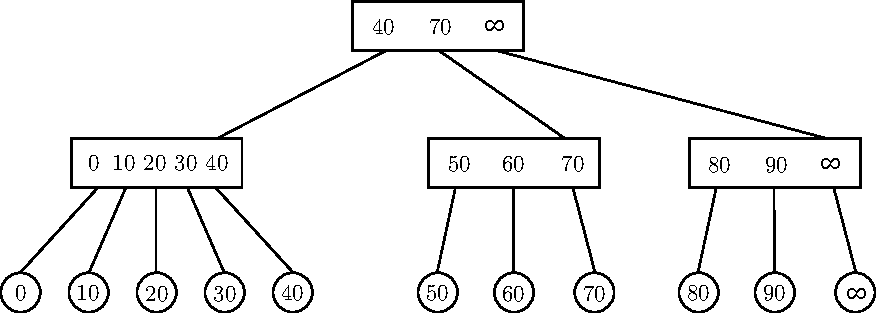
\includegraphics{pics/drawing.pdf}
\caption{Příkladový (3,5)-strom}
\end{figure}
	
Vkládáme \texttt{key, value}.  Pokud  je  strom  prázdný  vytvoříme  kořen,  který  bude  mít  nově  vkládaný záznam jako jednoho syna a vrchol s klíčem $\infty$ jako druhého syna. Začneme u kořene. Z vrcholu přejdeme na jeho syna, který má nejbližší vyšší klíč než \texttt{key}.

Po vložení zavoláme algoritmus vyvažování na otce nově vzniklého vnějšího vrcholu.
	
\subsection{Hledání}

Pokud hledáme podle klíče \texttt{key}, začneme v kořeni a sestupujeme na syny s nejbližším vyšším klíčem, nebo případně klíčem rovným \texttt{key}. Pokud nedojdeme do vnějšího vrcholu s hledaným klíčem, strom klíč neobsahuje.

\subsection{Mazání}

Pokud je třeba vrchol vymazat, nejdříve ho je třeba najít ve stromě a potom odstranit. Pokud byl navíc maximálním klíčem v některých vnitřních vrcholech, je třeba změnit v jeho předcích klíče na druhý nejvyšší vrchol v otci mazaného vrcholu (Takový musí existovat.)

Může být porušeno vyvážení stromu, proto je třeba zavolat vyvažování na bývalého otce smazaného vrcholu.
	
\subsection{Vyvažování}

Pokud jsme přidávali nebo mazali od posledního spuštění vyvažování pouze jeden vrchol, povolený počet synů ve vrcholech může být porušen o nejvýše 1.


	
\section{Analýza složitosti}
	
\lipsum[10]
	
\lipsum[10]
	
\listoffigures
\listoftables
\section*{Seznam příloh}
%\addcontentsline{toc}{chapter}{Seznam příloh}
\begin{enumerate}
	\item[A.] Zdrojový kód knihovny
	\item[B.] Zdrojové kódy příkladů
\end{enumerate}
\begin{thebibliography}{10}
	\bibitem{aocp}
	KNUTH, Donald Ervin. The Art of Computer Programming. Upper Saddle River, NJ: Addison-Wesley, 2011. ISBN 978-0321751041.
\end{thebibliography}
\end{document}